%% Type de document et encodage de la police
\documentclass[a4paper]{article}
\usepackage[utf8x]{inputenc}
\usepackage[T1]{fontenc}
\usepackage[french]{babel}

%% Initialise la taille des pages et des marges
\usepackage[a4paper, top=3cm, bottom=3cm, left=2cm, right=2cm, marginparwidth=2cm]{geometry}

%% Packs utiles
\usepackage{amsmath}
\usepackage{graphicx}
\usepackage{hyperref}
\usepackage{xcolor}
\usepackage{standalone}

%% Commandes perso
\renewcommand{\arraystretch}{1.2} %% row 20% longer

%% Pour les exemples
\usepackage{mdframed}
\newmdenv[topline=false, bottomline=false, rightline=false, skipabove=\topsep, skipbelow=\topsep]{example}

%% Pour les diagrammes
\usepackage{tikz}
\usetikzlibrary{calc, arrows}
\tikzstyle{description} = [
    anchor=north,
    text width=3.5cm,
    text centered,
]


\title{Computer Networking -- Simple Web Page Request}
\author{Grégoire Roumache}
\date{November 2019}


\begin{document}

\maketitle















\section{Connecting to the Internet}





Connecting your laptop to the internet and loading a webpage is a 4 steps process\footnote{Reference: Computer Networking A Top-Down Approach 6th Edition, by Kurose \& Ross.}\footnote{The icons come from \url{https://www.cisco.com/c/en/us/about/brand-center/network-topology-icons.html}.}:
\begin{enumerate}
    \item Get an IP address.
    \item Get the MAC address of the gateway.
    \item Get the IP address behind the domain name.
    \item Get the webpage (e.g. \texttt{www.google.com}).
\end{enumerate}















\section{Topology of the Network}





\begin{center}
\includestandalone{tikz-files/network-topology}
\end{center}















\section{Get an IP Address}





\begin{center}
    \begin{tikzpicture}
    
        %% images
        \node (laptop) [] at (0,0) {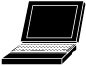
\includegraphics[width=1.5cm]{images/laptop.jpg}};
        \node (switch) [] at (5,0) {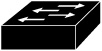
\includegraphics[width=1.5cm]{images/workgroup_switch.jpg}};
        \node (router) [] at (10,0) {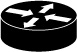
\includegraphics[width=1.5cm]{images/router.jpg}};
    
        %% descriptions
        \node (laptop-description) [anchor=north, text width=3.5cm, text centered] at (0,-1) {laptop \\ \texttt{08:00:27:97:91:D1} \\ \;};
        \node [anchor=north, text width=3cm, text centered] at (5,-1) {switch};
        \node (router-description) [anchor=north, text width=3.5cm, text centered] at (10,-1) {router \\ \texttt{08:00:27:11:90:3E} \\ \texttt{68.85.2.1}};
    
        %% links
        \draw[<->] (laptop) -- (switch);
        \draw[<->] (router) -- (switch);
    
        %%%%%%%%%%%%%%%%%%%%%%%%%%%%%%%%%%%%%%%%%%%%%%%%%%%%%%%%%%%%%%%%%%%%%%%%%%
    
        %% DHCP Request
        \draw [->, blue] (laptop) to [out=-45, in=-135] node[anchor=north]{Which IP should I use?} (router);
        \draw [->, red] (router-description) to [out=-135, in=-45] node[anchor=north]{\texttt{68.85.2.101}} (laptop-description);
    
    \end{tikzpicture}
\end{center}





We connect our laptop to the school's network with an Ethernet cable. In order to communicate over the internet, we have to get an IP address. This is done with the DHCP protocol.





%% Protocole Internet (TCP/IP) --- DHCP Request
\begin{center}
    \begin{tikzpicture}
        
        %% Numbers
        \node [minimum height=1cm] at (0,0) {\textbf{5}};
        \node [minimum height=1cm] at (0,-1) {\textbf{4}};
        \node [minimum height=1cm] at (0,-2) {\textbf{3}};
        \node [minimum height=1cm] at (0,-3) {\textbf{2}};
        \node [minimum height=1cm] at (0,-4) {\textbf{1}};

        %% Rectangles
        \node [anchor=west, text width=2.5cm, text centered, minimum height=1cm, rectangle, draw=black] at (0.5,0) {\textbf{Application}};
        \node [anchor=west, text width=2.5cm, text centered, minimum height=1cm, rectangle, draw=black] at (0.5,-1) {\textbf{Transport}};
        \node [anchor=west, text width=2.5cm, text centered, minimum height=1cm, rectangle, draw=black] at (0.5,-2) {\textbf{Network}};
        \node [anchor=west, text width=2.5cm, text centered, minimum height=1cm, rectangle, draw=black] at (0.5,-3) {\textbf{Data Link}};
        \node [anchor=west, text width=2.5cm, text centered, minimum height=1cm, rectangle, draw=black] at (0.5,-4) {\textbf{Physical}};

        %% Protocols
        \node (dhcp) [anchor=west, text width=3cm, text centered, minimum height=1cm] at (3.25,0) {\textcolor{red}{\textbf{DHCP Request}}};
        \node (udp) [anchor=west, text width=3cm, text centered, minimum height=1cm] at (3.25,-1) {UDP Segment};
        \node (ip) [anchor=west, text width=3cm, text centered, minimum height=1cm] at (3.25,-2) {IP Datagram};
        \node (ethernet) [anchor=west, text width=3cm, text centered, minimum height=1cm] at (3.25,-3) {Ethernet Frame};
        \node (physical) [anchor=west, text width=3cm, text centered, minimum height=1cm] at (3.25,-4) {Electrical Signals};

        %% Arrows
        \draw [->] ($(dhcp.east) + (0,-0.05)$) to [out=-60, in=60] ($(udp.east) + (0,0.05)$);
        \draw [->] ($(udp.east) + (0,-0.05)$) to [out=-60, in=60] ($(ip.east) + (0,0.05)$);
        \draw [->] ($(ip.east) + (0,-0.05)$) to [out=-60, in=60] ($(ethernet.east) + (0,0.05)$);
        \draw [->] ($(ethernet.east) + (0,-0.05)$) to [out=-60, in=60] ($(physical.east) + (0,0.05)$);

        %% UDP Segment
        \node (UdpPorts) [anchor=west] at (8,-0.5) {\begin{tabular}{ll} source port: 68 & dhcp client \\ destination port: 67 & dhcp server \end{tabular}}; 
        \draw ($(UdpPorts.north west) + (0.5,0)$) -- (UdpPorts.north west) -- (UdpPorts.south west) -- ($(UdpPorts.south west) + (0.5,0)$);

        %% IP Datagram
        \node (IPDatagram) [anchor=west] at (8,-2) {\begin{tabular}{l} source IP address: \texttt{0.0.0.0} \\ destination IP address: \texttt{255.255.255.255} \end{tabular}}; 
        \draw ($(IPDatagram.north west) + (0.5,0)$) -- (IPDatagram.north west) -- (IPDatagram.south west) -- ($(IPDatagram.south west) + (0.5,0)$);

        %% Ethernet Frame
        \node (EthernetFrame) [anchor=west] at (8,-3.5) {\begin{tabular}{l} source MAC address: \texttt{08:00:27:97:D1} \\ destination MAC address: \texttt{FF:FF:FF:FF:FF:FF} \end{tabular}};
        \draw ($(EthernetFrame.north west) + (0.5,0)$) -- (EthernetFrame.north west) -- (EthernetFrame.south west) -- ($(EthernetFrame.south west) + (0.5,0)$);

        %% link to the explanations
        \draw[->] ($(udp.east) + (0.25,0)$) -- ($(udp.east) + (1.25,0)$);
        \draw[->] ($(ip.east) + (0.25,0)$) -- ($(ip.east) + (1.25,0)$);
        \draw[->] ($(ethernet.east) + (0.25,0)$) -- ($(ethernet.east) + (1.25,0)$);

    \end{tikzpicture}
\end{center}




Process:
\begin{enumerate}
    \item The \textcolor{blue}{\textbf{laptop}}'s OS creates a \textbf{DHCP Request} which is put inside a \textbf{UDP Segment}, which is put inside an \textbf{IP Datagram}, which is put inside an \textbf{Ethernet Frame}, which is transformed into electrical signals and sent over the cable.
    \item The \textcolor{blue}{\textbf{switch}} receives the ethernet frame, which has a broadcast destination address (\texttt{FF:FF:FF:FF:FF:FF}), and transmits it on all ongoing ports, including the port connected to the router.
    \item The \textcolor{blue}{\textbf{router}} receives the ethernet frame.
    \begin{enumerate}
        \item since the destination address of the internet frame is a broadcast (\texttt{FF:FF:FF:FF:FF:FF}), it extracts the IP datagram
        \item since the IP datagram has a broadcast destination address (\texttt{255.255.255.255}), it demultiplexes the UDP segment
        \item since the destination port is 67, the router opens a DHCP process and reads the DHCP Request message
    \end{enumerate}
    \item The \textcolor{blue}{\textbf{router}} sends back a response:
    \begin{enumerate}
        \item the DHCP server creates a \textbf{DHCP ACK message} that contains the IP addresses of the laptop, the DNS, the default gateway and the subnet block (or the netmask)
        \item the DHCP message is put inside a UDP segment, which is put inside an IP datagram, which is put inside an Ethernet frame.
    \end{enumerate}



%% Internet Protocol (TCP/IP) --- DHCP ACK
\begin{center}
    \begin{tikzpicture}
        
        %% Numbers
        \node [minimum height=1cm] at (0,0) {\textbf{5}};
        \node [minimum height=1cm] at (0,-1) {\textbf{4}};
        \node [minimum height=1cm] at (0,-2) {\textbf{3}};
        \node [minimum height=1cm] at (0,-3) {\textbf{2}};
        \node [minimum height=1cm] at (0,-4) {\textbf{1}};

        %% Rectangles
        \node [anchor=west, text width=2.5cm, text centered, minimum height=1cm, rectangle, draw=black] at (0.5,0) {\textbf{Application}};
        \node [anchor=west, text width=2.5cm, text centered, minimum height=1cm, rectangle, draw=black] at (0.5,-1) {\textbf{Transport}};
        \node [anchor=west, text width=2.5cm, text centered, minimum height=1cm, rectangle, draw=black] at (0.5,-2) {\textbf{Network}};
        \node [anchor=west, text width=2.5cm, text centered, minimum height=1cm, rectangle, draw=black] at (0.5,-3) {\textbf{Data Link}};
        \node [anchor=west, text width=2.5cm, text centered, minimum height=1cm, rectangle, draw=black] at (0.5,-4) {\textbf{Physical}};

        %% Protocols
        \node (dhcp) [anchor=west, text width=3cm, text centered, minimum height=1cm] at (3.25,0) {\textcolor{red}{\textbf{DHCP ACK}}};
        \node (udp) [anchor=west, text width=3cm, text centered, minimum height=1cm] at (3.25,-1) {UDP Segment};
        \node (ip) [anchor=west, text width=3cm, text centered, minimum height=1cm] at (3.25,-2) {IP Datagram};
        \node (ethernet) [anchor=west, text width=3cm, text centered, minimum height=1cm] at (3.25,-3) {Ethernet Frame};
        \node (physical) [anchor=west, text width=3cm, text centered, minimum height=1cm] at (3.25,-4) {Electrical Signals};

        %% Arrows
        \draw [->] ($(dhcp.east) + (0,-0.05)$) to [out=-60, in=60] ($(udp.east) + (0,0.05)$);
        \draw [->] ($(udp.east) + (0,-0.05)$) to [out=-60, in=60] ($(ip.east) + (0,0.05)$);
        \draw [->] ($(ip.east) + (0,-0.05)$) to [out=-60, in=60] ($(ethernet.east) + (0,0.05)$);
        \draw [->] ($(ethernet.east) + (0,-0.05)$) to [out=-60, in=60] ($(physical.east) + (0,0.05)$);

        %% DHCP ACK
        \node (DhcpAck) [anchor=west] at (8,0) {\begin{tabular}{l} IP address: \texttt{68.85.2.101} \\ DNS: \texttt{68.87.71.226} \\ subnet block: \texttt{68.85.2.0/24} \end{tabular}};
        \draw ($(DhcpAck.north west) + (0.5,0)$) -- (DhcpAck.north west) -- (DhcpAck.south west) -- ($(DhcpAck.south west) + (0.5,0)$);

        %% UDP Segment
        % \node (UdpPorts) [anchor=west] at (8,-1) {\begin{tabular}{ll} source port: 67 & dhcp server \\ destination port: 68 & dhcp client \end{tabular}};
        % \draw ($(UdpPorts.north west) + (0.5,0)$) -- (UdpPorts.north west) -- (UdpPorts.south west) -- ($(UdpPorts.south west) + (0.5,0)$);

        %% IP Datagram
        \node (IPDatagram) [anchor=west] at (8,-2) {\begin{tabular}{l} source IP address: \texttt{68.85.2.1} \\ destination IP address: \textcolor{blue}{\textbf{IDK...}} \end{tabular}};
        \draw ($(IPDatagram.north west) + (0.5,0)$) -- (IPDatagram.north west) -- (IPDatagram.south west) -- ($(IPDatagram.south west) + (0.5,0)$);

        %% Ethernet Frame
        % \node (EthernetFrame) [anchor=north west] at (8,-3.6) {\begin{tabular}{l} source MAC address: \texttt{08:00:27:11:90:3E} \\ destination MAC address: \texttt{08:00:27:97:D1} \end{tabular}};
        % \draw ($(EthernetFrame.north west) + (0.5,0)$) -- (EthernetFrame.north west) -- (EthernetFrame.south west) -- ($(EthernetFrame.south west) + (0.5,0)$);

        %% link to the explanations
        \draw[->] ($(dhcp.east) + (0.15,0)$) -- ($(DhcpAck.west) + (-0.25,0)$);
        % \draw[->] ($(udp.east) + (0.15,0)$) -- ($(udp.east) + (1.25,0)$);
        \draw[->] ($(ip.east) + (0.15,0)$) -- ($(IPDatagram.west) + (-0.25,0)$);
        % \draw[->] ($(ethernet.east) + (0.15,0)$) -- ($(EthernetFrame.west) + (-0.25,0)$);

    \end{tikzpicture}
\end{center}



    \item The \textcolor{blue}{\textbf{switch}} receives the ethernet frame. It reads the destination address (\texttt{08:00:27:97:91:D1}) and sends it to the corresponding laptop because it \textit{learned} on which port this interface is connected.
    \item The \textcolor{blue}{\textbf{laptop}} receives the ethernet frame.
    \begin{enumerate}
        \item it extracts the IP datagram, the UDP segment and, finally, the DHCP ACK message
        \item it stores its IP address as well as the DNS's IP address
        \item it installs the IP address of the default gateway into its \textit{IP forwarding table}.
    \end{enumerate}
\end{enumerate}















\section{Get the MAC Address of the Gateway}





The laptop can't access the internet if it can't send an ethernet frame to the gateway. That's why the next step is to get its the MAC address.





%% ARP Protocol --- ARP Query
\begin{center}
    \begin{tikzpicture}
        
        %% Numbers
        \node [minimum height=1cm] at (0,-1) {\textbf{3}};
        \node [minimum height=1cm] at (0,-2) {\textbf{2}};
        \node [minimum height=1cm] at (0,-3) {\textbf{1}};

        %% Rectangles
        \node [anchor=west, text width=2.5cm, text centered, minimum height=1cm, rectangle, draw=black] at (0.5,-1) {\textbf{Network}};
        \node [anchor=west, text width=2.5cm, text centered, minimum height=1cm, rectangle, draw=black] at (0.5,-2) {\textbf{Data Link}};
        \node [anchor=west, text width=2.5cm, text centered, minimum height=1cm, rectangle, draw=black] at (0.5,-3) {\textbf{Physical}};

        %% Protocols
        \node (arp) [anchor=west, text width=3cm, text centered, minimum height=1cm] at (3.25,-1) {\textcolor{red}{\textbf{ARP Query}}};
        \node (ethernet) [anchor=west, text width=3cm, text centered, minimum height=1cm] at (3.25,-2) {Ethernet Frame};
        \node (physical) [anchor=west, text width=3cm, text centered, minimum height=1cm] at (3.25,-3) {Electrical Signals};

        %% Arrows
        \draw [->] ($(arp.east) + (0,-0.05)$) to [out=-60, in=60] ($(ethernet.east) + (0,0.05)$);
        \draw [->] ($(ethernet.east) + (0,-0.05)$) to [out=-60, in=60] ($(physical.east) + (0,0.05)$);

        %% Ethernet Frame
        \node (EthernetFrame) [anchor=west] at (8,-2) {\begin{tabular}{l} source MAC address: \texttt{08:00:27:97:91:D1} \\ destination MAC address: \texttt{FF:FF:FF:FF:FF:FF} \end{tabular}};
        \draw ($(EthernetFrame.north west) + (0.5,0)$) -- (EthernetFrame.north west) -- (EthernetFrame.south west) -- ($(EthernetFrame.south west) + (0.5,0)$);

        %% link to the explanations
        \draw[->] ($(ethernet.east) + (0.25,0)$) -- ($(ethernet.east) + (1.25,0)$);

    \end{tikzpicture}
\end{center}





Process:
\begin{enumerate}
    \item The \textcolor{blue}{\textbf{laptop}} creates an \textbf{ARP Query}, put it inside an \textbf{Ethernet Frame}, sends it to the \textcolor{blue}{\textbf{switch}}. Since this is a broadcast destination address (\texttt{FF:FF:FF:FF:FF:FF}), it transmits it on all ongoing ports.
    \item The \textcolor{blue}{\textbf{router}} (= gateway) receives the ethernet frame, extracts the ARP Query and see that the IP address in the query is the same as its interface's address.
    \item The \textcolor{blue}{\textbf{router}} sends back a response:
    \begin{enumerate}
        \item it creates an \textbf{ARP Reply} indicating that the MAC address corresponding to: \texttt{68.85.2.1}, is: \texttt{08:00:27:11:90:3E}
        \item the ARP reply is put inside an ethernet frame and sent over to the \textcolor{blue}{\textbf{switch}}, which sends it to the \textcolor{blue}{\textbf{laptop}}.
    \end{enumerate}
\end{enumerate}





%% ARP Protocol --- ARP Reply
\begin{center}
    \begin{tikzpicture}

        %% Numbers
        \node [minimum height=1cm] at (0,-1) {\textbf{3}};
        \node [minimum height=1cm] at (0,-2) {\textbf{2}};
        \node [minimum height=1cm] at (0,-3) {\textbf{1}};

        %% Rectangles
        \node [anchor=west, text width=2.5cm, text centered, minimum height=1cm, rectangle, draw=black] at (0.5,-1) {\textbf{Network}};
        \node [anchor=west, text width=2.5cm, text centered, minimum height=1cm, rectangle, draw=black] at (0.5,-2) {\textbf{Data Link}};
        \node [anchor=west, text width=2.5cm, text centered, minimum height=1cm, rectangle, draw=black] at (0.5,-3) {\textbf{Physical}};

        %% Protocols
        \node (arp) [anchor=west, text width=3cm, text centered, minimum height=1cm] at (3.25,-1) {\textcolor{red}{\textbf{ARP Reply}}};
        \node (ethernet) [anchor=west, text width=3cm, text centered, minimum height=1cm] at (3.25,-2) {Ethernet Frame};
        \node (physical) [anchor=west, text width=3cm, text centered, minimum height=1cm] at (3.25,-3) {Electrical Signals};

        %% Arrows
        \draw [->] ($(arp.east) + (0,-0.05)$) to [out=-60, in=60] ($(ethernet.east) + (0,0.05)$);
        \draw [->] ($(ethernet.east) + (0,-0.05)$) to [out=-60, in=60] ($(physical.east) + (0,0.05)$);

        %% ARP Query
        \node (ArpQuery) [anchor=west] at (8,-0.75) {\begin{tabular}{l} IP address: \texttt{68.85.2.1} \\ MAC address: \texttt{08:00:27:11:90:3E} \end{tabular}}; 
        \draw ($(ArpQuery.north west) + (0.5,0)$) -- (ArpQuery.north west) -- (ArpQuery.south west) -- ($(ArpQuery.south west) + (0.5,0)$);

        %% Ethernet Frame
        \node (EthernetFrame) [anchor=west] at (8,-2.25) {\begin{tabular}{l} source MAC address: \texttt{08:00:27:11:90:3E} \\ destination MAC address: \texttt{08:00:27:97:91:D1} \end{tabular}};
        \draw ($(EthernetFrame.north west) + (0.5,0)$) -- (EthernetFrame.north west) -- (EthernetFrame.south west) -- ($(EthernetFrame.south west) + (0.5,0)$);

        %% link to the explanations
        \draw[->] ($(arp.east) + (0.25,0)$) -- ($(arp.east) + (1.25,0)$);
        \draw[->] ($(ethernet.east) + (0.25,0)$) -- ($(ethernet.east) + (1.25,0)$);

    \end{tikzpicture}
\end{center}















\section{Find the IP Address of the Website}





The user of the laptop wants to get on the website: \texttt{www.google.com}. But the computer needs an IP address. In order to translate the domain name to an IP address, it will contact the DNS.





%% Protocole Internet (TCP/IP) --- DNS Query Message
\begin{center}
    \begin{tikzpicture}
        
        %% Numbers
        \node [minimum height=1cm] at (0,0) {\textbf{5}};
        \node [minimum height=1cm] at (0,-1) {\textbf{4}};
        \node [minimum height=1cm] at (0,-2) {\textbf{3}};
        \node [minimum height=1cm] at (0,-3) {\textbf{2}};
        \node [minimum height=1cm] at (0,-4) {\textbf{1}};

        %% Rectangles
        \node [anchor=west, text width=2.5cm, text centered, minimum height=1cm, rectangle, draw=black] at (0.5,0) {\textbf{Application}};
        \node [anchor=west, text width=2.5cm, text centered, minimum height=1cm, rectangle, draw=black] at (0.5,-1) {\textbf{Transport}};
        \node [anchor=west, text width=2.5cm, text centered, minimum height=1cm, rectangle, draw=black] at (0.5,-2) {\textbf{Network}};
        \node [anchor=west, text width=2.5cm, text centered, minimum height=1cm, rectangle, draw=black] at (0.5,-3) {\textbf{Data Link}};
        \node [anchor=west, text width=2.5cm, text centered, minimum height=1cm, rectangle, draw=black] at (0.5,-4) {\textbf{Physical}};

        %% Protocols
        \node (dns) [anchor=west, text width=3cm, text centered, minimum height=1cm] at (3.25,0) {\textcolor{red}{\textbf{DNS Query}}};
        \node (udp) [anchor=west, text width=3cm, text centered, minimum height=1cm] at (3.25,-1) {UDP Segment};
        \node (ip) [anchor=west, text width=3cm, text centered, minimum height=1cm] at (3.25,-2) {IP Datagram};
        \node (ethernet) [anchor=west, text width=3cm, text centered, minimum height=1cm] at (3.25,-3) {Ethernet Frame};
        \node (physical) [anchor=west, text width=3cm, text centered, minimum height=1cm] at (3.25,-4) {Electrical Signals};

        %% Arrows
        \draw [->] ($(dns.east) + (0,-0.05)$) to [out=-60, in=60] ($(udp.east) + (0,0.05)$);
        \draw [->] ($(udp.east) + (0,-0.05)$) to [out=-60, in=60] ($(ip.east) + (0,0.05)$);
        \draw [->] ($(ip.east) + (0,-0.05)$) to [out=-60, in=60] ($(ethernet.east) + (0,0.05)$);
        \draw [->] ($(ethernet.east) + (0,-0.05)$) to [out=-60, in=60] ($(physical.east) + (0,0.05)$);

        %% DNS Query
        \node (DnsQuery) [anchor=west] at (8,0) {\begin{tabular}{l} Query section: \texttt{www.google.com} \end{tabular}};
        \draw ($(DnsQuery.north west) + (0.5,0)$) -- (DnsQuery.north west) -- (DnsQuery.south west) -- ($(DnsQuery.south west) + (0.5,0)$);

        %% UDP Segment
        \node (UdpPorts) [anchor=west] at (8,-1) {\begin{tabular}{ll} destination port: 53 & (dns server) \end{tabular}}; 
        \draw ($(UdpPorts.north west) + (0.5,0)$) -- (UdpPorts.north west) -- (UdpPorts.south west) -- ($(UdpPorts.south west) + (0.5,0)$);

        %% link to the explanations
        \draw[->] ($(dns.east) + (0.25,0)$) -- ($(dns.east) + (1.25,0)$);
        \draw[->] ($(udp.east) + (0.25,0)$) -- ($(udp.east) + (1.25,0)$);

    \end{tikzpicture}
\end{center}





Note that the destination IP address is that of the DNS server \textbf{but} the destination MAC address of the Ethernet frame is that of the gateway.





\begin{enumerate}





%% Gateway
\item The \textcolor{blue}{\textbf{router}} receives the ethernet frame. It extracts the IP datagram, checks its forwarding table and decide to send it over to the internet provider's network. \textbf{Note}: the data link's frame is changed, even the protocol used could different.





%% Internet Provider
\item The \textcolor{blue}{\textbf{internet provider's router}} receives the frame, extracts the IP datagram and decide to send it over to the DNS server from its forwarding table.





%% DNS Server
\item The \textcolor{blue}{\textbf{DNS server}} receives the IP datagram and extracts the DNS query message and it sends back the \textbf{DNS reply} with the IP address of \texttt{google.com}: \texttt{64.233.169.105}.





%% Laptop
\item The \textcolor{blue}{\textbf{laptop}} finally receives the IP address of the server of \texttt{google.com}.





\end{enumerate}















\section{Get the Website's Page}





The protocol used to get the website's page is \textbf{HTTP} and it's located on the application layer. \textbf{But} we can't just send the \textbf{HTTP GET} message directly. Firstly, we have to open a \textbf{TCP} (transport layer) connection with a three-way handshake.

In the end, Google's server will send the \textbf{HTTP response} and the laptop's browser will display the webpage.








\end{document}
